% Fig 3 — campaign flow with GPU-hour economics, standalone TikZ.
% Compile: pdflatex -interaction=nonstopmode fig3_campaign_flow.tex
% Style matches fig1_architecture.tex. Numbers trace to docs/24 (+§3.4),
% docs/22 §5 (STOP-gate), docs/23 (audit), docs/26 (Phase 5.6 seeds);
% GPU-h economics per docs/25 §5 row 9 (~270 saved vs ~66 spent on the arc).
\documentclass[tikz,border=10pt]{standalone}
\usetikzlibrary{positioning,arrows.meta,calc}

\definecolor{spat}{HTML}{2A78D6}   % controlled campaign / re-tests
\definecolor{freq}{HTML}{E34948}   % STOP-gate / falsification
\definecolor{estc}{HTML}{4A3AA7}   % pre-registration / frozen rules
\definecolor{advc}{HTML}{52514E}   % audit
\definecolor{ink}{HTML}{0B0B0B}
\definecolor{ink2}{HTML}{52514E}
\definecolor{muted}{HTML}{898781}
\definecolor{okgreen}{HTML}{2E7D32} % verdict

% W2 (m-50 / CEL-13): base font bumped one step — at IEEE Access column
% width the previous \footnotesize body rendered below the template minimum.
\newcommand{\head}{\normalsize\bfseries}
\newcommand{\body}{\small}

\begin{document}
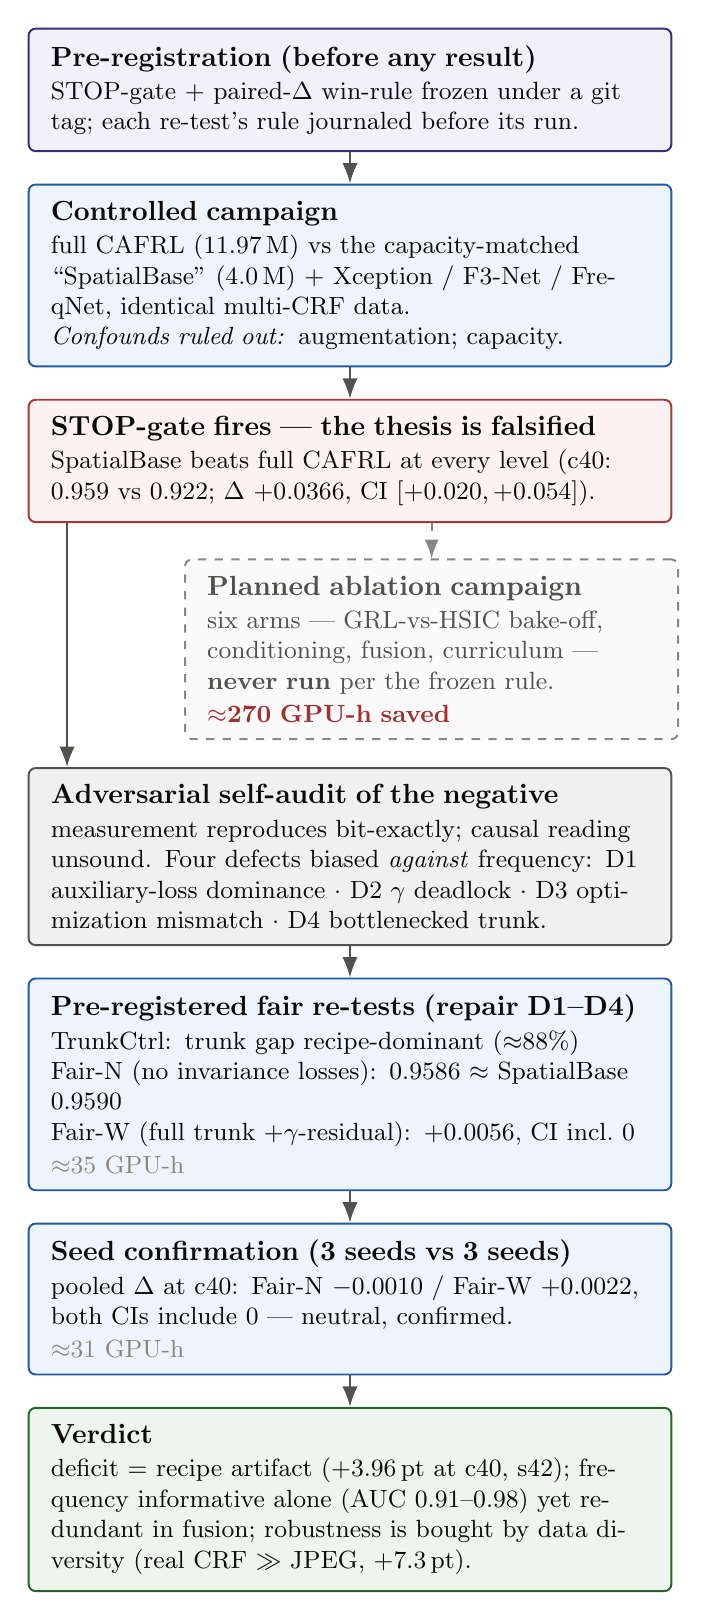
\begin{tikzpicture}[
  font=\small,
  every node/.style={text=ink},
  stage/.style={draw, rounded corners=2.5pt, align=left, text width=7.6cm,
                inner xsep=8pt, inner ysep=6pt, line width=0.7pt},
  preblock/.style={stage, draw=estc!75!black, fill=estc!7},
  runblock/.style={stage, draw=spat!75!black, fill=spat!8},
  stopblock/.style={stage, draw=freq!75!black, fill=freq!7},
  audblock/.style={stage, draw=advc, fill=black!6},
  verblock/.style={stage, draw=okgreen!80!black, fill=okgreen!8},
  ghost/.style={stage, draw=muted, dashed, fill=black!2, text=ink2},
  flow/.style={-{Latex[length=2.6mm]}, line width=0.8pt, draw=ink2},
  ghostflow/.style={-{Latex[length=2.4mm]}, line width=0.7pt, draw=muted, dashed},
]

% ---------------------------------------------------------------- stages ----
\node[preblock] (prereg) at (0,0) {%
  {\head Pre-registration (before any result)}\\[1pt]
  {\body STOP-gate $+$ paired-$\Delta$ win-rule frozen under a git tag;
   each re-test's rule journaled before its run.}};

\node[runblock, below=4mm of prereg] (campaign) {%
  {\head Controlled campaign}\\[1pt]
  {\body full CAFRL (11.97\,M) vs the capacity-matched
   ``SpatialBase'' (4.0\,M) $+$ Xception / F3-Net / FreqNet, identical
   multi-CRF data.\\
   \textit{Confounds ruled out:} augmentation; capacity.}};

\node[stopblock, below=4mm of campaign] (stop) {%
  {\head STOP-gate fires --- the thesis is falsified}\\[1pt]
  {\body SpatialBase beats full CAFRL at every level
   (c40: 0.959 vs 0.922; $\Delta$ +0.0366, CI [+0.020,\,+0.054]).}};

\node[ghost, below right=4.5mm and -62mm of stop, text width=5.7cm] (ablations) {%
  {\head\color{ink2} Planned ablation campaign}\\[1pt]
  {\body six arms --- GRL-vs-HSIC bake-off, conditioning, fusion, curriculum ---
   \textbf{never run} per the frozen rule.\\[1pt]
   \color{freq!70!black}\textbf{$\approx$270 GPU-h saved}}};

\node[audblock, anchor=north] (audit) at ($(stop.south -| stop.center)+(0,-3.1cm)$) {%
  {\head Adversarial self-audit of the negative}\\[1pt]
  {\body measurement reproduces bit-exactly; causal reading unsound.
   Four defects biased \emph{against} frequency: D1 auxiliary-loss
   dominance $\cdot$ D2 $\gamma$ deadlock $\cdot$ D3 optimization
   mismatch $\cdot$ D4 bottlenecked trunk.}};

\node[runblock, below=4mm of audit] (retests) {%
  {\head Pre-registered fair re-tests (repair D1--D4)}\\[1pt]
  {\body TrunkCtrl: trunk gap recipe-dominant ($\approx$88\%)\\
   Fair-N (no invariance losses):
   0.9586 $\approx$ SpatialBase 0.9590\\
   Fair-W (full trunk $+\gamma$-residual): +0.0056, CI incl.\ 0\\[1pt]
   {\color{muted}$\approx$35 GPU-h}}};

\node[runblock, below=4mm of retests] (seeds) {%
  {\head Seed confirmation (3 seeds vs 3 seeds)}\\[1pt]
  {\body pooled $\Delta$ at c40: Fair-N $-$0.0010 / Fair-W +0.0022,
   both CIs include 0 --- neutral, confirmed.\\[1pt]
   {\color{muted}$\approx$31 GPU-h}}};

\node[verblock, below=4mm of seeds] (verdict) {%
  {\head Verdict}\\[1pt]
  {\body deficit $=$ recipe artifact ($+3.96$\,pt at c40, s42); frequency
   informative alone (AUC 0.91--0.98) yet redundant in fusion; robustness is
   bought by data diversity (real CRF $\gg$ JPEG, $+7.3$\,pt).}};

% ----------------------------------------------------------------- edges ----
\draw[flow] (prereg.south) -- (campaign.north);
\draw[flow] (campaign.south) -- (stop.north);
\draw[ghostflow] (stop.south -| ablations.north) -- (ablations.north);
\draw[flow] ([xshift=5mm]stop.south west) -- ([xshift=5mm]audit.north west);
\draw[flow] (audit.south) -- (retests.north);
\draw[flow] (retests.south) -- (seeds.north);
\draw[flow] (seeds.south) -- (verdict.north);


\end{tikzpicture}
\end{document}
